\documentclass[letterpaper, 12pt]{article}
\usepackage[letterpaper, top=2.5cm, bottom=2.5cm, left=3cm, right=3cm]{geometry} %margenes
\usepackage[backend=biber]{biblatex}\addbibresource{bibliografia.bib} %manejo de bibliografía (BORRAR SI NO ES NECESARIO)
\usepackage[utf8]{inputenc} %manejo de caracteres especiales
\usepackage[spanish]{babel} %manejo de encabezados de inglés a español
\usepackage{fancyhdr} %formato de los encabezados de página
\usepackage{ragged2e} %alineado real justficado
\usepackage{graphicx} %manejo de imagenes
\usepackage{amsmath} %manejo de notación matemática
\usepackage{mathtools} %manejo de notación matemática
\usepackage{blindtext} %texto de relleno
\usepackage{amssymb} %manejo de simbología
\usepackage{float} %centrado de imaene
\usepackage{hyperref} %manejo de enlaces e hipervínculos

\hypersetup{
  colorlinks   = true, %Colours links instead of ugly boxes
  urlcolor     = blue, %Colour for external hyperlinks
  linkcolor    = blue, %Colour of internal links
  citecolor   = red %Colour of citations
}

\pagestyle{fancy}
\fancyhf{}
\rfoot{\thepage}

\nocite{*}

\begin{document}
    
    %PORTADA
    \begin{titlepage}
        \begin{figure}[ht]
            \centering
            
\includegraphics[width=15cm]{logosITT.png}
        \end{figure}
        \centering
        {\scshape\LARGE Tecnológico Nacional de México\\Instituto Tecnológico de Tijuana\par}
        \vspace{1cm}
        {\scshape\Large Fundamentos de Bases de Datos\par}
        \vspace{1cm}
        {\scshape\Large Unidad 1\par}
        \vspace{1.5cm}
        {\huge\bfseries Diferencias, Objetivos y Usos de las Bases de Datos\par}
        \vspace{2cm}
        {\Large\itshape C. Abraham Jhared Flores Azcona\\19211640\par}
        \vfill
        Profesora: \par
        M.C. María Magdalena Serrano Ortega
    
        \vfill

        {\large 26 de febrero de 2021}
    \end{titlepage}

    %indices
    \newpage
        \thispagestyle{empty}
        \tableofcontents %indice de contenidos
        \listoffigures %indice de figuras

    %cuerpo
    \newpage
    \begin{justify}
        \setcounter{page}{1}
        \thispagestyle{fancy}
        \lhead{\textbf{Diferencias, Objetivos y Usos de las Bases de Datos}}
        \section{Introducción}
        \justify
        En esta breve investigación, se expoenen las bases de datos a gran escala para obtener una noción elemental de las mismas. De manera más concreta qué és y qué no és una base de datos, sus tipos, sus objetivos y sus usos y aplicaciones generales y particulares.
        \section{Diferencia entre una base de datos y un sistema de archivos}
        \justify
        A pesar de la indiscutible diferencia gramatical, llega el caso en que se puede confundir a dichos temas como tal. En esta sección se explican sus definiciones y respectivas diferencias.
            \subsection{Base de datos}
        \justify
        A grandes rasgos, una base de datos es simple y sencillamente una colección de información estructurada tipicamente almacenada de manera
        electrónica en un sistema computacional. El ícono común para las bases de datos se muestra a continuación en el siguiente diagrama:
        \begin{figure}[H]
            \centering
            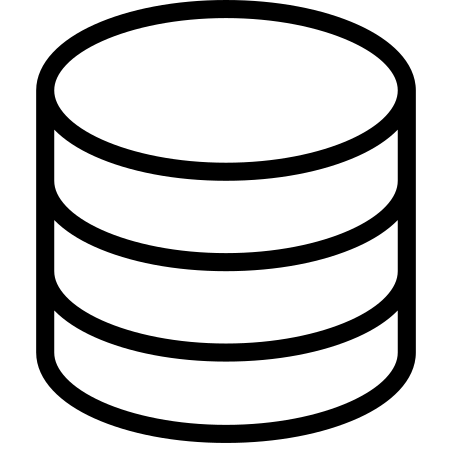
\includegraphics[width=5cm,height=4cm]{database_icon.png}
            \caption{Icono alusivo de una base de datos.}
        \end{figure}
        Los tipos de bases de datos son los siguientes:
        \begin{itemize}
            \item \textbf{Relacionales:} dominantes en los 80's. Provee la manera más eficiente y flexible de acceder a información estructurada.
            \item \textbf{Orientada a Objetos:} su información es representada en la forma de objetos, como en POO.
            \item \textbf{Distribuidas:} consisten en dos o más archivos localizados en distintos lugares.
            \item \textbf{Depositos de datos:} consiste en ser un repositorio central de datos pensada para busquedas y análisis rápidas.
            \item \textbf{NoSQL:} también conocida como \emph{no-relacional.} Permite a datos no-estructurados y semi-estructurados ser almacenados y manipulados.
            \item \textbf{De Grafos:} almacena datos en términos de entidades y las relaciones entre las mismas.
            \item \textbf{OLTP:} base de datos analítica y rápida diseñada para grandes cantidades de transacciones realizadas por múltiples usuarios. 
            \item \textbf{\emph{Open Source:}} aquella la cual su código fuente es disponible para el interesadoñ pueden ser bases SQL ó NoSQL.
            \item \textbf{De nube:} colección de datos, estructurados o no-estructurados que residen en una plataforma de cómputo en la nube pública, privada o híbrida.
            \item \textbf{Multimodelo:} combina disitintos tipos de modelos de bases de datos en un \emph{backend} único e integrado.
            \item \textbf{Documentación/JSON:} para almacenar, retirar y administrar información orientada a documentos. Manera moderna de almacenar datos en formato JSON.
            \item \textbf{Autónomas:} la más reciente. Son de base de cómputo en la nube y usan aprendizaje de máquina para automatizar la depuración, seguridad, repaldo, actualización y
            otras rutinas correpondientes a los deberes administrativos previamente realizados por administradores de bases de datos.
        \end{itemize}
            \subsection{Sistema de archivos}
        \justify
        Se le refiere también como \emph{administración de archivos}. Este es un método que permite organizar y extraer archivos de un medio de almacenamiento (como un disco duro).
        Estos usualmente consisten de archivos separado en grupos llamados \emph{directorios}. Estos directorios pueden contener archivos o directorios adicionales.
        \\\newline
        Sin un sistema de archivos, todos los archivos no tendrían organización y sería imposible para que un archico con el mismo nombre pudiese existir. Generalmente se administran los
        archivos con una jerarquía, que nos permite ver archivos en el directorio actual y despues navegar hacia cualquier subdirectorio.
        \begin{figure}[H]
            \centering
            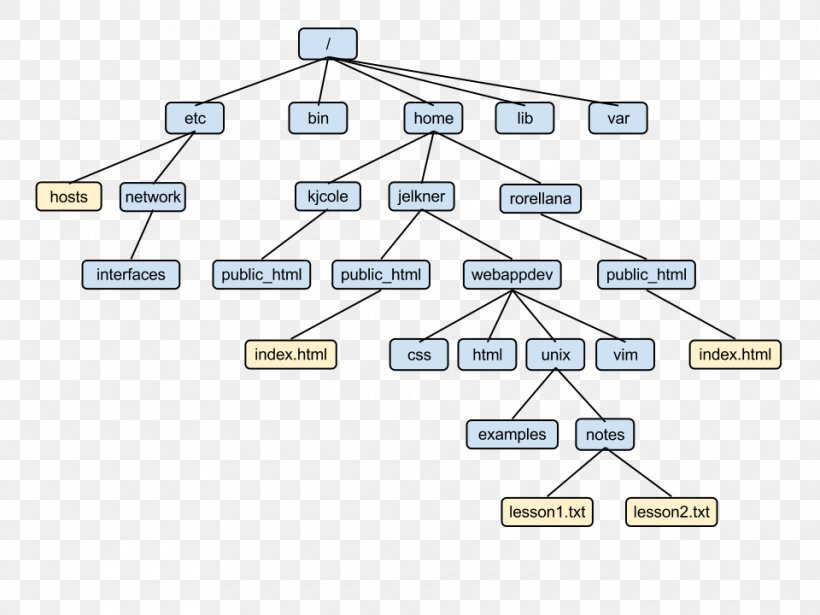
\includegraphics[width=10cm,height=5.6cm]{sistemaarchivo.jpg}
            \caption{Estructura de directorios del sistema de archivos UNIX.}
        \end{figure}
        Algunos ejemplos de los sistemas de archivos son los siguientes:
        \begin{itemize}
            \item \textbf{FAT}: usado principalmente en las memorias USB Flash. %computerhope: FAT
            \item \textbf{GFS}: desarrollado por la Universidad de Minnesota. Este se extiende a través de una porción pequeña de un disco duro y permite a distintas computadoras actuar como una sola maquinaria. %computerhope: GFS 
            \item \textbf{HFS}: usado para almacenar archivos en los disquettes, discos DC-ROM y discos duros de computadoras viejas de Apple Macintosh. Ya no se usa en computadoras Apple con OS X. %computerhope: hfs
            \item \textbf{NTFS}: usado para el manejo de archivos en los sistemas operativos Microsoft Windows NT, Windows 2000, Windows XP, Windows 7 y Windows 10. Provee mejores métodos de protección y recuperación de datos. %computerhope: NTFS
            \item \textbf{UDF}: desarrollado en 1995 por la Asociación de Tecnología de Almacenamiento Optico (OSTA, por sus siglas en inglés). Comunmente usado con CD y DVD. Es soportado por todos los sistemass operativos. %computerhope: UDF
        \end{itemize}
            \subsection{Diferencias}
            \justify
        La principal diferencia entre las base de datos y un sistema de archivos es que las bases de datos solo almacenan los datos previamente estructurados mientras que los sistemas de archivos
        acomodan archivos y en base a los directorios poder acceder a ellos. En otras palabras las bases de datos almacenan datos mientras que los sistemas de archivos permiten su acceso.
        \section{Objetivos de una base de datos}
        \justify
        Cuando se habla de los objetivo de una base de datos, se interpolan los objetivos de administración. En concreto, los objetivos principales son los siguientes:
        \begin{itemize}
            \item \textbf{Disponibilidad de datos.}
            \item \textbf{Integridad de datos.}
            \item \textbf{Seguridad de datos.}
            \item \textbf{Independencia de datos.}
        \end{itemize}
        \subsection{Disponibilidad de datos}
        \justify
        Define el grado y la extensión a la cual los datos están listos para usarse con las tecnologías de la información y los procedimientos administrativos, herramientas y tecnologías requeridas para permitir,
        manejar y continuar la disponibilidad de los datos. También se refiere a la adquisición de datos popr el sistema. Aparte, también se refiere a como se pueden arrojar dato de distintas fuentes, distintos tipos y distintos formatos, incluyendo
        la conversión de formatos que se conviertan en parte de un proyecto. Muchos de los datos deben de ser procesados previamente antes de formar parte de la base de datos.
        \\\newline
        En resumen, la disponibilidad de datos se refiere a que los mismo estén disponibles:
        \begin{itemize}
            \item A una gran variedad de usuarios.
            \item En un formato significativo.
            \item A un costo razonable.
            \item Con facilidad de acceso.
            \item Cuando y donde se requiera.
        \end{itemize}
        \subsection{Integridad de datos}
        \justify
        Se refiere a la correctitud de los datos en la base de datos. En otras palabras, que tan confiables son los datos disponibles en la base de datos. También sigifica que los datos sean auténticos, acertados y consistentes. Es el mantenimiento y reaseguranza
        de la presición y consistencia de los datos en su ciclo de vida. Se implementa por un diseño apropiado, y autenticando a los mismos usando rutinas de revisión de errores y de validación. Un ejemplo de esto, para mantener la integridad de filas y columnas numéricas
        no deben aceptar datos alfabéticos.
        \\\newline
        Este objetivo también se interpola con la seguridad de datos. En resumen, las prácticas que permiten asegurar la integridad de datos incluyen:
        \begin{itemize}
            \item Encripción de datos, la cual asegura los datos por encripción.
            \item Respaldo de datos, la cual almacena una copia de datos en un lugar alternativo.
            \item Control de acceso, incluyendo la asignación de privilegios de lectura y sobreescritura.
            \item Validación de entrada, para prevenir la escritura de datos incorrectos.
            \item Validación de datos, para certificar una transmición no corrompida.
        \end{itemize}
        \subsection{Seguridad de datos}
        \justify
        Se refiere a las medidas de protección de privacidad digital que son aplicadas para prevenir el acceso no autorizado a computadoras, sitios web, bases de datos o parte de las mismas. También incluye el hecho de que solo los usuarios autorizados puedan acceder a los datos. Este objetivo
        se puede aplicar con contraseñas. Se protegen a los datos de posibles corrupciones, incluyendo las medidas colectivas usadas para proteger y asegurar a la base de datos y sus programas de administración.
        \\\newline
        En resumen, este objetivo se logra procurando lo siguiente:
        \begin{itemize}
            \item Evitar almacenar información delicada en la nube.
            \item Leer los terminos y politicas de privacidad y manejo de datos.
            \item Tomarse enserio las contraseñas.
            \item Encriptar.
            \item Usar un servicio de cómputo en la nube que sea encriptado.
        \end{itemize}
        \subsection{Independencia de datos}
        \justify
        Se refiere a la facilidad de compartir la base de datos por actuales y futuras aplicaciones. Esto incluye a la facilidad con la cual los metadatos pueden ser actualizados sin afectar a los datos mismos. Si se realizan cambios al formato de la tabla, esto no debe cambiar los datos que residen en el dispositivo
        de almacenamiento.
        \\\newline
        En resumen, la independencia de datos permite:
        \begin{itemize}
            \item Cambiar la base de datos sin afectar los programas de aplicación.
            \item Cambiar el hardware o el software del sistema sin afectar los programas de aplicación.
            \item Compartir los datos de distinas aplicaciones provisto de perspectivas apropiadas para la aplicación.
            \item Control de redundancia.
            \item Evitar duplicados.
        \end{itemize} 
        \section{Usos y aplicaciones de las bases de datos}
        \justify
        Como cualquier herramienta versatil, contiene distintas aplicaciones en distintos ámbitos. Por el afán de la brevedad se exponen tres casos particulares.
        \subsection{Contabilidad}
        \justify
        En un sistema contable se utiliza una aplicación personalizada de una base de datos para manejar los datos financieros. Las formas personalizadas son usadas para grabar
        activos, pasivos, inventario y las transacciones entre los clientes y los proveedores. Los estados de cuenta, hojas de balanza, ordenes de compra y comunicados generados son reportes
        personalizados basados en la información que ha entrado en la base de datos. Sus aplicaciones contables pueden realizarse en una computadora acomodada para un pequeño negocio o en un 
        ambiente de red compartida para acomodar las necesidades de múltiples departamentos y localizaciones en organizaciones más grandes. 
        \\\newline
        Ejemplos de sistemas contables hechos en aplicaciones de bases de datos son:
        \begin{itemize}
            \item \textbf{Microsoft Money.}
            \item \textbf{Quicken.}
            \item \textbf{QuickBooks.}
            \item \textbf{Peachtree.}
        \end{itemize} 
        \subsection{Administración de relaciones con el consumidor}
        \justify
        Esta aplicación se refiere a la base de datos la cual ha sido personalizada para administrar mercadotécnia, ventas y apoyar las relaciones entre el negocio y los clientes. La última finalidad
        es la de maximizar ventas, minimizar costos y tratar relaciones estratégicas con los cliente. Programas como \textbf{ACT}, o el administrador de deberes en \textbf{Outlook} pueden ser personalizados para
        acomodar las necesidades de los individuos y de negocios pequeños. \textbf{SAP}, \textbf{Salesforce.com} y \textbf{Siebel} son aplicaciones de bases de datos robustas pensadas para empresas grandes.
        \subsection{La Web}
        \justify
        Muchos sitios web son construidos usando ciertas aplicaciones de bases de datos simultaneamente como componentes nucleare. Muchas de las tiendas de supermercado incluyendo
        \emph{Bestbuy.com},  \emph{Amazon.com} usan bases de datos para almacenar, actualizar y presentar datos sobre los porducto en venta. Estos sitios web tambiéen combinan una base de datos
        contable para registrar transacciones de ventas una aplicación base de datos ARC para incorporar la retroalimentación y conducir a una experiencia positiva del consumidor. La popular aplicación basada
        en la aplicación web \emph{Facebook} es esencialmente una base de datos hecha sobre el sistema \textbf{MySQL} y es un indicador del uso incrementado de aplicaciones de bases de datos como pilares de
        aplicaciones basadas en la web.

        \section{Conclusión} %minimo de 100 palabras!!!
        \justify
        Como se ha expuesto a lo largo de esta investigación breve, conocer los aspectos que le son caraterísticos a las bases de datos son sumamente importantes para poder trabajar con ellas desde su teoría hasta su practica. Saber sus diferencias 
        con los sistemas de archivos nos permite evitar confusiones e inclusive errores en el estudio de las base de datos como en sus respectivas aplicaciones en la vida real, aunque es relevante decir que no está de más conocer las características 
        de los sistemas de archivos para complementar las base de datos y poderse auxiliar de las mismas si llegara el momento de. Sus principios son de mucha ayuda conocer para tener en cuenta la indiscutible reponsabilidad que se tiene al estudiar y, 
        en un futuro no muy lejano, trabajar con ellas mantener los estándaresy el profesionalismo que se espera de nosotros. Y finalmente conocer los usos y aplicaciones permite tener posibles ideas para sus implementaciones. 

    \end{justify}

    %bibliografía
    \fancypagestyle{myplain} %estilo personalizado para la bibliografia
    {
      \fancyhf{}
      \renewcommand\headrulewidth{0pt}
      \renewcommand\footrulewidth{0pt}
      \fancyfoot[R]{\thepage}
    } %sin la barrita ni los encabezados, solo el numero de página en el pie derecho

    \newpage
        \thispagestyle{myplain} %ponerlo como \thispagestyle{myplain}
        \addcontentsline{toc}{section}{Referencias}
        \printbibliography
\end{document}